

\section{CARACTERÍSTICAS: Suficientable}

En este curso se presenta una visión general de cómo programar un computador, incluyendo las relaciones que existen entre el programa y la máquina (el software y el hardware), los pasos en la creación de los programas y particularidades de diferentes lenguajes de programación.

El computador nos proporciona aquella información requerida por nosotros que quizás sin él sería inalcanzable, pero la máquina por sí sola no lo hace, por su cuenta no resuelve problemas comerciales, ni problemas científicos, ni de ningún tipo. Mientras no le suministremos una serie detallada de instrucciones para que nos resuelva esos problemas y nos brinde la información que buscamos, el computador es sencillamente una curiosidad de mucho valor que, en vez de ser útil, estorba.

\section{OBJETIVOS GENERALES DEL CURSO}

Al finalizar este curso, el estudiante:

\begin{itemize}
	\item Tendrá bases lógicas y técnicas para la programación de un computador 

	\item Poseerá conocimientos suficientes que le permitirán organizar y escribir instrucciones para un computador, es decir, programarlo de una manera eficaz mediante la utilización de un lenguaje de programación

	\item Erradicará la creencia que llevan algunas personas de que la programación es privilegio sólo de pocos, y así se sentirá bastante satisfecho de tener un computador a "sus órdenes"

	\item Comprenderá que no saber programar un computador, implica una merma, en un gran porcentaje, del producto del trabajo realizado con el mismo, a pesar del software tan desarrollado existente en el mercado
\end{itemize}

Texto Guia \cite{farrell2011programming}

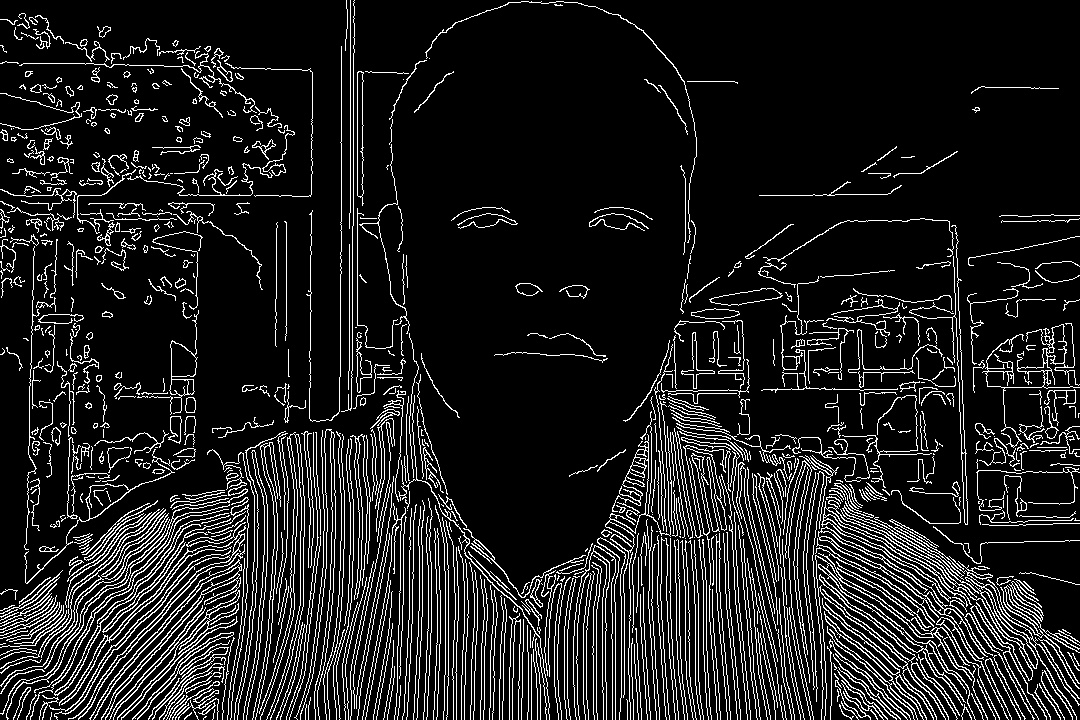
\includegraphics[width=15cm]{SamCanny.jpg}
